\chapter{【淮南王】}
\begin{wrapfigure}{r}{0.3\textwidth}
\centering
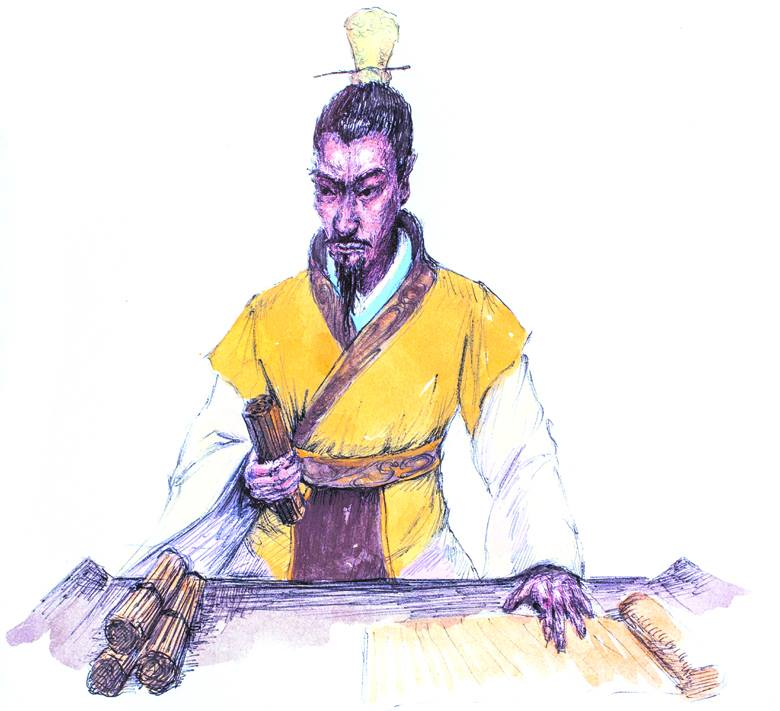
\includegraphics[width=0.3\textwidth]{pics/p002.jpg}
\vspace{-25pt}
\caption{淮南王}
%\label{test}
\end{wrapfigure}

$\cdots\cdots$ 發明豆腐 $\cdots$ 「一人得道,雞犬升天」 $\cdots\cdots$
\footnote{摘自{\Kai《讀者》}雜誌2015年11月號,圖/李發友}


讀{\Kai《史記》}如讀小說,輕鬆、好玩,而且耐人尋味。
沛縣的混混劉邦得了天下,分封諸王,異姓的倒有幾個有名的,
還都讓他給廢了,從此立個臭規矩,非劉氏不王。
可是,自家孩子封的王,大抵籍籍無名,
都是混吃等死的主兒,唯一例外的是淮南王。

第一任淮南王劉長,說起來有點來路不明。
他的母親,原是漢初異姓王趙王張敖的美人,
諸姬妾之一,後來劉邦過境,張敖為了拍劉邦的馬屁,
把美人送給劉邦侍寢。這樣的事,此前有,此後也沒斷了。

但凡款待牛人或者上司,送個美人給嘗嘗鮮,就跟送金銀玉帛一樣稀鬆平常。
牛人睡過之後,揚長而去,就當什麼事也沒發生。
這樣的美人禮物,可以送張三,也可以送李四,當然也可以自己享用。
所以,即使有了孩子,也未必能知道是誰的。那年月又沒有DNA鑒定,誰能說得清?

但是,張敖的美人,自打為劉邦侍寢之後,居然懷孕了,
而被張敖斷定為劉邦的種,不再染指,供了起來,直到生下龍子,
或者說是他認為的龍子。等到趙王張敖連同妻妾一併被劉邦找茬收了,
這件事便被有司得知,彙報上去。劉邦也不加理會,顯然是不大相信。
美人的兄弟託關係找到呂后身邊的寵臣審食其,審食其將此事告訴了呂后。
呂后當然不會喜歡劉邦身邊再多一個美女,自然一言不發,審食其當然也就只好算了。

沒想到,這個就為劉邦侍寢一次的美人,居然憤而自殺。
她這一死,讓劉邦相信了這個孩子可能真的是他留的種。
於是,劉邦就又多了一個兒子劉長。
待到原來的淮南王英布被劉邦逼得造反而被滅掉,
劉長就成了淮南王。

這個劉長,幼年喪母,卻長得很結實,力氣很大,能扛鼎,估計也喜歡舞槍弄棒的。
對他娘的死,他一直耿耿於懷。其實,他娘的死,該賴他的爹。
但那時的人怎麼敢恨自己的父親,於是就遷怒於辟陽侯審食其。

劉長長大以後,已經是漢文帝的天下了,一日,他袖裡藏著一枚鐵錘,
找上審食其的門去,光天化日之下一錘就將這位侯爺給打倒了,
然後讓人將其腦袋割下。然後,劉長大模大樣地到皇帝那兒去請罪,
說是請罪,卻說了一大串審食其的罪過。這個劉長,見了皇帝,
不稱陛下,只叫「大兄」的。這個皇帝還能把他怎麼樣呢?
只好打發他回家了。

這樣的慣法,任是好人也慣壞了。
不久,就傳來淮南王僭用天子儀仗,擅為法令,意欲謀反的消息。
諸大臣一致要求將其處以極刑,漢文帝法外開恩,只是將他發配了。
封在一輛大車裡,直奔目的地,途中不許地方官開封。
受不了這種羞辱的劉長,不食而死。當然沒準兒,是給憋死、餓死的。

劉長死了,民間輿論卻批評皇帝。
民謠曰:「一尺布,尚可縫。一斗粟,尚可舂。兄弟二人,不能相容。」
為了平息議論,證明自己並非貪圖淮南的土地,
漢文帝將淮南故地分成三份,給了淮南王的三個兒子。
其中仍封為淮南王的,是劉安。

後面的淮南王,封地少了,愛好卻多了。劉安的名氣在漢代諸王中堪稱第一,
他好讀書、彈琴,好神仙,好與文士交往,還好美食。門下眾多文雅之士,
一起編了一套{\Kai《淮南子》},為中國傳統文化的傳承,加分不少。

據說,淮南王劉安的另一大貢獻,是發明了豆腐。但估計這豆腐的發明,
跟{\Kai《淮南子》}一樣,也是集體的力量,起作用的無名之輩,
無法考證,只好都記在了劉安的名下。
都說中國人有四大發明,其實四大發明之外,豆腐和馬鐙兩個,
也算是重大發明,亞洲各國吃豆腐,都是拜淮南王之賜。
據說,歐美人對豆腐越來越感興趣,中國人在那邊實在混不下去了,
只要有做豆腐的手藝,就可以發點小財。

有這麼多愛好和發明的淮南王跟他的父親一樣,最後還是因為謀反丟了性命。
漢代做諸王的,也真是不容易,一個不留神,就成了反賊。
沒辦法,漢代的皇帝制度,還沒有嫡長子傳承的規矩,
所以跟皇帝同樣血緣的人,有錢、有地,還有兵,怎麼都是麻煩。
真反假反不好說,但反正大家都沒個好結果。

不過這回,民間沒有傳歌謠,而是傳出一種說法,
說劉安其實沒死,而是吃了仙藥,升天去了。
神仙給的仙藥量比較大,不僅自己吃了,而且他們家的雞犬也一併吃了,
一同飛升,到天上快活去了。
從此留下一句俗語,叫作「一人得道,雞犬升天」。

民間總是愛跟皇帝唱反調,沒法子。

